%\begin{titlepage}%ambiente que permite a criação de uma capa própria
\begin{center}   %modo centralizado

\begin{figure}[h] %h insere a figura onde ela está no texto
\centering        %centraliza a figura

\includegraphics[width=7.0cm, height=3.0cm]{imagens/UNIGRAN.jpg} %define o
% tamanho da figura
\end{figure}      %encerra modo figura

\textbf{CENTRO UNIVERSITÁRIO DA GRANDE DOURADOS}

\begin{figure}[h]
\centering
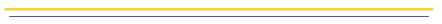
\includegraphics[width=15.0cm, height=0.40cm]{imagens/AMARELO.jpg}
\end{figure}

\textbf{MARCELO BENTO PEREIRA} 
\\

\vspace{5cm}%define os espaços entre as frases de 7 centímetros

\textbf{VOZ SOBRE IP: UMA PROPOSTA DE MELHORIA DO TELEATENDIMENTO EMERGENCIAL DA POLÍCIA MILITAR DE DOURADOS UTILIZANDO PABX IP} %\textbf Texto em negrito

\vspace{10cm}

\begin{figure}[h]
\centering
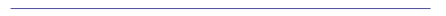
\includegraphics[width=15.0cm, height=0.40cm]{imagens/AZUL.jpg}

\end{figure}

\textbf{Dourados}
\vspace{-0,5cm} %diminue os espaço entre as frases em 0,5 centímetros a menos que o normal

\textbf{2015}

\end{center}%encerra modo centralizado
%\end{titlepage}%encerra modo de capa